\documentclass{article}

\usepackage[margin=0.5in]{geometry}
\usepackage{multicol}
\usepackage{siunitx}
\usepackage{tikz}
\usetikzlibrary{quotes,angles}

\title{Plane Geometry Set A}
\date{}
\author{}

\begin{document}
\maketitle
\noindent Problems should be solved without calculators unless otherwise specified.
Remember to explain how you solved a problem.
\begin{multicols}{2}
    \begin{enumerate}
        \item In quadrilateral $ABCD$, the measure of angle $A$ is half the sum of the measures of the other angles.
            What is the measure of angle $A$?
            Express your answer to the nearest integer.
            \vspace{3cm}
        \item The two circles in the figure are tangent at $G$.
            Prove that $m\angle E = m\angle F$.
            \begin{center}
                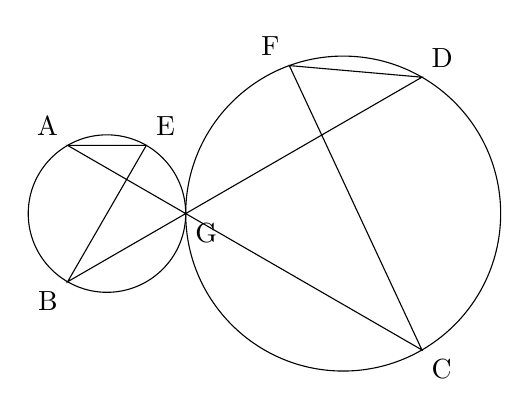
\begin{tikzpicture}
                    \draw (0,0) circle (1cm);
                    \coordinate[label=above left:A] (A) at (120:1);
                    \coordinate[label=below left:B] (B) at (240:1);
                    \coordinate[label=above right:E] (E) at (60:1);
                    \coordinate[label=below right:G] (G) at (1,0);
                    \begin{scope}[shift={(3,0)}]
                        \draw (0,0) circle (2cm);
                        \coordinate[label=above left:F] (F) at (110:2);
                        \coordinate[label=above right:D] (D) at (60:2);
                        \coordinate[label=below right:C] (C) at (300:2);
                    \end{scope}
                    \draw (A) -- (E) -- (B) -- (G) -- (D) -- (F) -- (C) -- (G) -- cycle;
                \end{tikzpicture}
            \end{center}
            \vspace{3cm}
        \item Triangle $ABC$ is inscribed in a semicircle as shown.
            If $m\angle ABC = \ang{24}$, what is the degree measure of $\angle BCA$?
            \begin{center}
                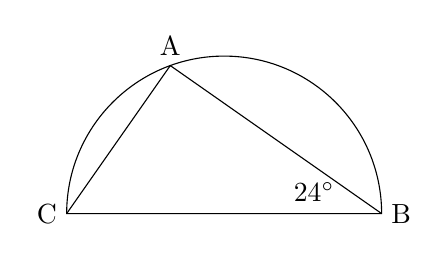
\begin{tikzpicture}
                    \draw (2,0) arc (0:180:2cm) -- cycle;
                    \coordinate[label=above:A] (A) at (110:2);
                    \coordinate[label=right:B] (B) at (2,0);
                    \coordinate[label=left:C] (C) at (-2,0);
                    \draw (A) -- (B) (A) -- (C);
                    \pic["$\ang{24}$", angle radius=1.5cm] {angle=A--B--C};
                \end{tikzpicture}
            \end{center}
            \vspace{3cm}
        \item In the figure, given that $m\angle ABC = \ang{60}$ and $m\angle BCD = \ang{70}$, find $m\angle CBD$.
            \begin{center}
                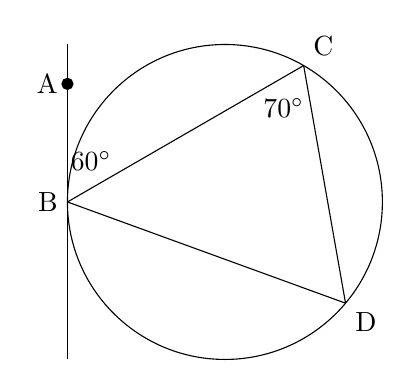
\begin{tikzpicture}
                    \draw (-2,-2) -- (-2,2);
                    \draw (0,0) circle (2cm);
                    \filldraw (-2,1.5) circle (2pt);
                    \coordinate[label=left:A] (A) at (-2, 1.5);
                    \coordinate[label=left:B] (B) at (-2,0);
                    \coordinate[label=above right:C] (C) at (60:2);
                    \coordinate[label=below right:D] (D) at (320:2);
                    \draw (B) -- (C) (C) -- (D) (B) -- (D);
                    \pic["$\ang{60}$", angle radius=1cm] {angle=C--B--A};
                    \pic["$\ang{70}$", angle radius=1cm] {angle=B--C--D};
                \end{tikzpicture}
            \end{center}
            \vspace{3cm}
        \item Segments $PA$ and $PT$ are tangent to the circle.
            Find the measure of $\angle TXA$ if $m\angle P = \ang{42}$.
            \begin{center}
                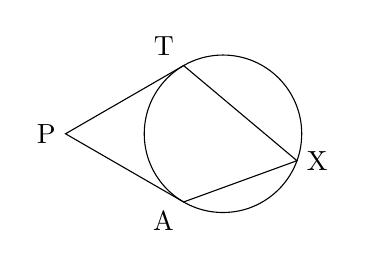
\begin{tikzpicture}
                    \draw (0,0) circle (1cm);
                    \coordinate[label=above left:T] (T) at (120:1);
                    \coordinate[label=left:P] (P) at (180:2);
                    \coordinate[label=below left:A] (A) at (240:1);
                    \coordinate[label=right:X] (X) at (340:1);
                    \draw (T) -- (P) -- (A) -- (X) -- cycle;
                \end{tikzpicture}
            \end{center}
            \vspace{3cm}
    \end{enumerate}
\end{multicols}
\end{document}
